\section{Results}
% Delete the text and write your Results here:
%------------------------------------
The results presented here are still undergoing a certain amount of work. Results are all given with a tolerance of below $3\%$ this corresponds to the following condition :

\begin{align} 
    (\Delta T, \Delta g, \Delta \mu) \leq 3\% \\
    \Delta T + \Delta g + \Delta \mu \leq 3\%
\end{align}

With the delta sign here corresponding to percent difference between exorem and exoris.\par

\Cref{fig:P_T} Shows the linkage between internal and atmosphere model, we see that no visible discontinuities are observable, confirming the linkage methods validity. We also observe that higher internal temperature exorem profiles tend to give temperature profiles that reach higher temperatures at the planetary center. While this might seem trivial, it does indicate that the linkage is indeed helping to resolve the internal structure.\par

\begin{figure}
    \centering
    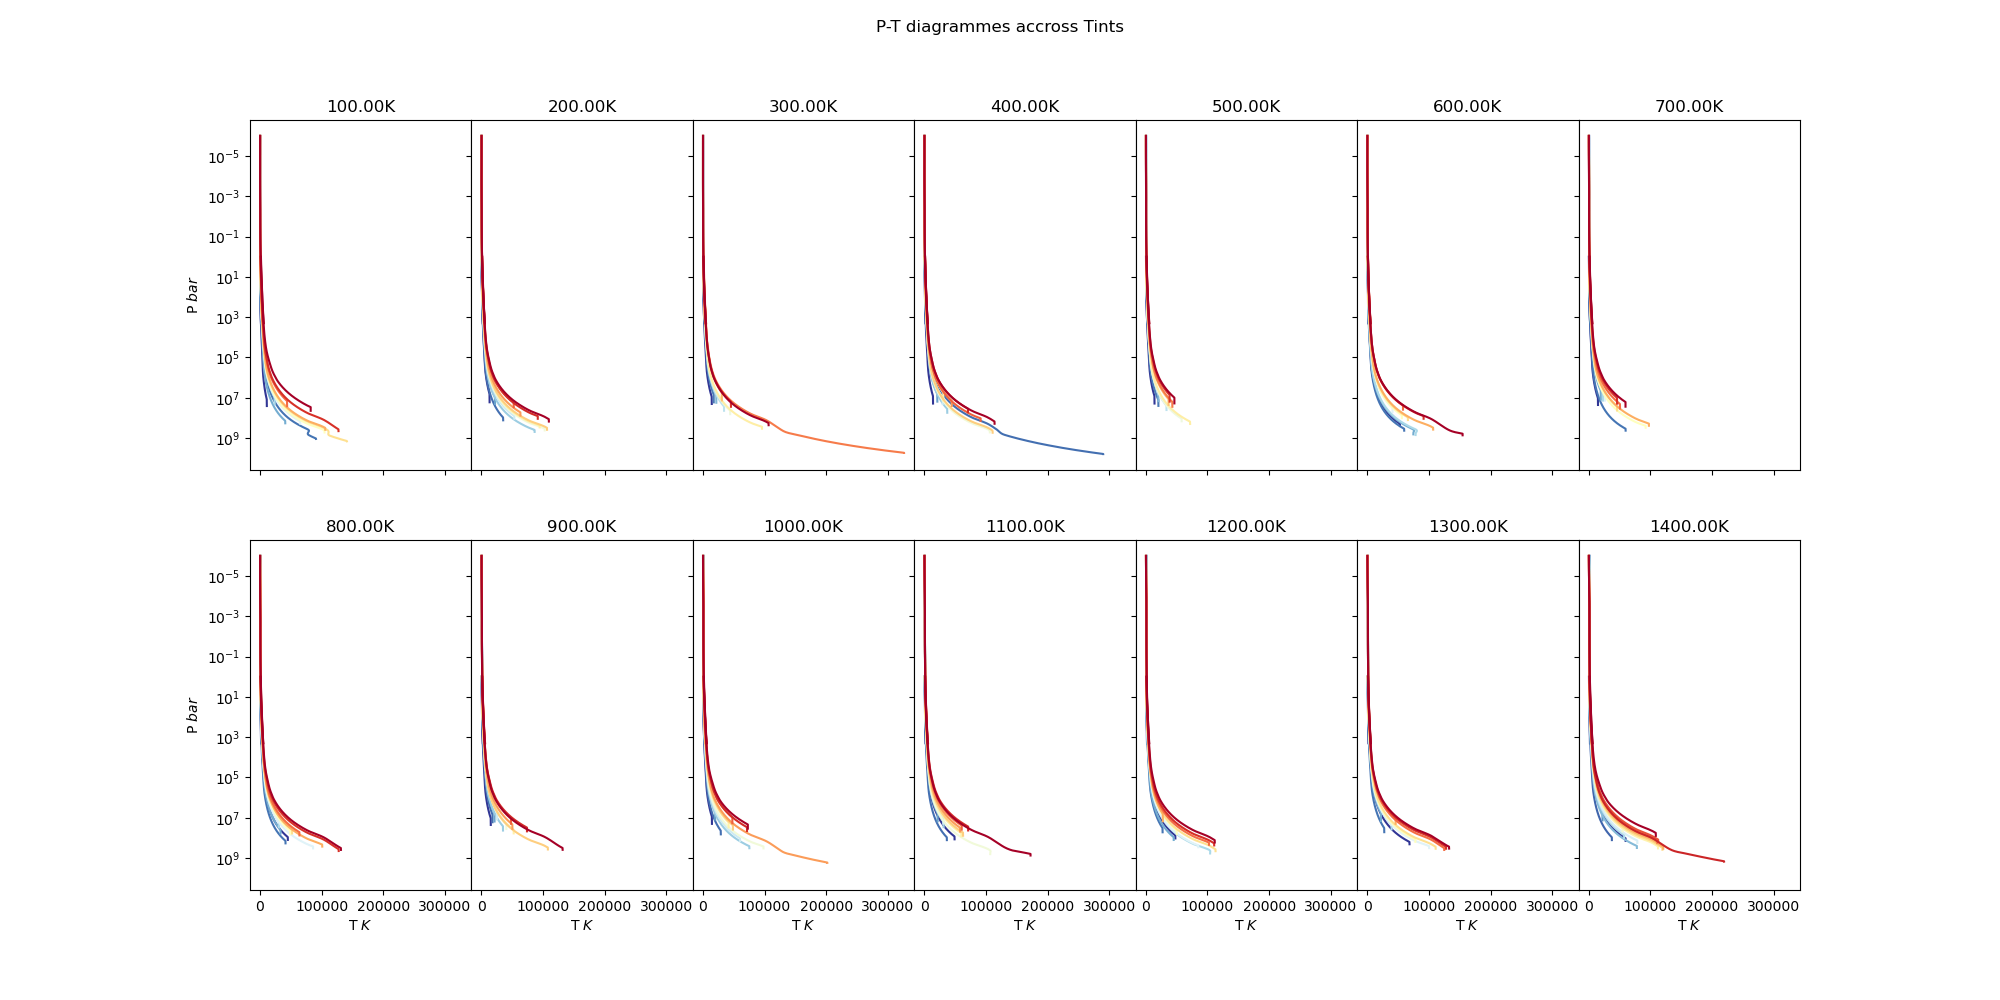
\includegraphics[width=0.48\textwidth]{Images/P_T.png}
    \caption{Pressure temperature profiles each plot at a given irradiation temperature and each profile at a given internal temperature}
    \label{fig:P_T}
\end{figure}

\Cref{fig:M_R_Tint} Shows how the radius is affected by mass, internal temperature and irradiation temperature. We see that higher internal temperatures lead to larger radii. High mass and high internal temperatures lead to a smaller radius than low mass and high temperature. While low temperature and high mass has only a small increase in radius compared to low mass and low internal temperature. It is hard to distinguish differences between different irradiation temperatures from these figures. \par

\begin{figure}
    \centering
    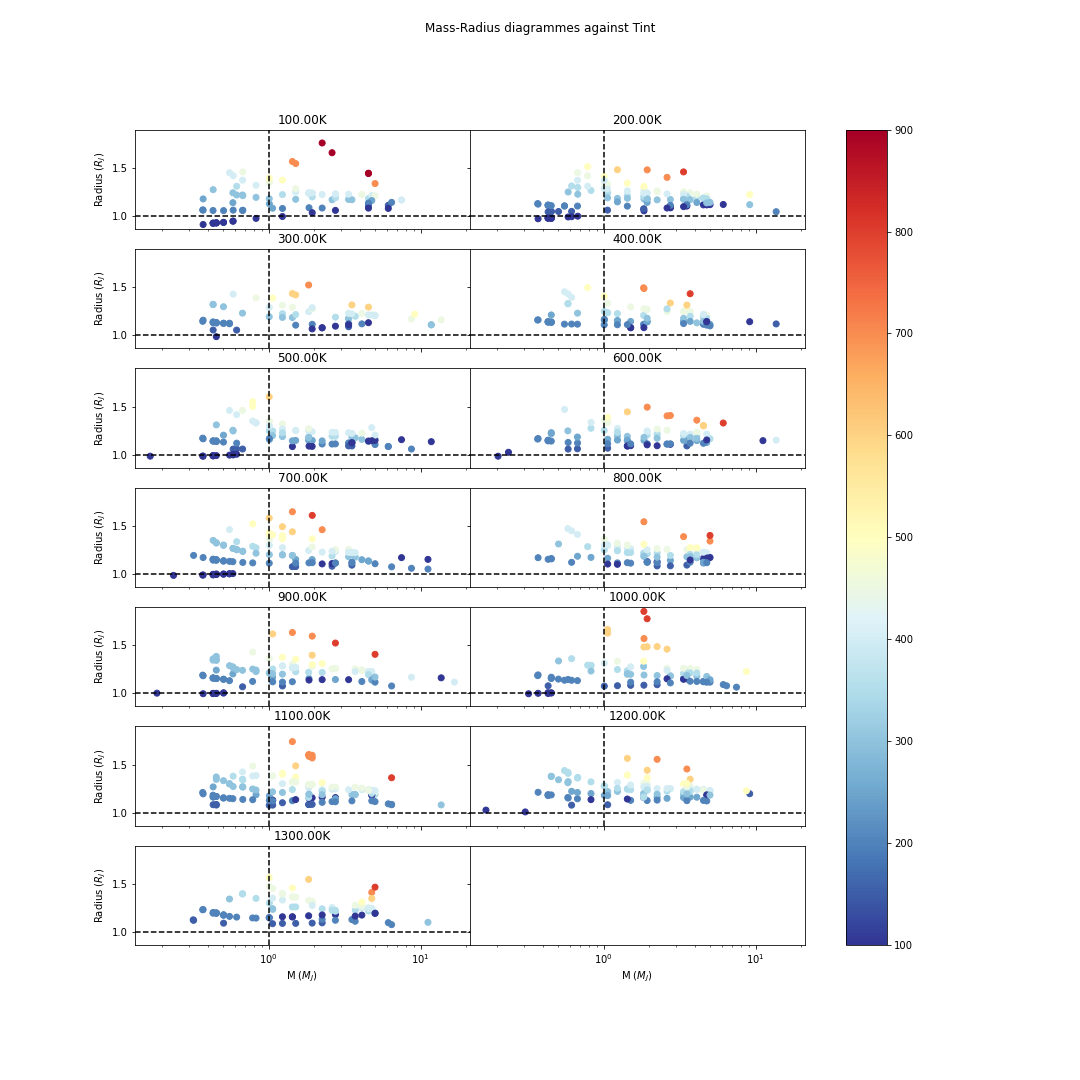
\includegraphics[width=0.48\textwidth]{Images/M_R_Tint.png}
    \caption{Mass Radius plots for different irradiation temperatures, plotted with internal temperature in color axis}
    \label{fig:M_R_Tint}
\end{figure}

\Cref{fig:M_R_Teff} Shows how the radius varies with the effective temperature of the planet. This figure is similar to \cref{fig:M_R_Tint}. The differences are that at high irradiation temperature, the effective temperature is given nearly entirely by the irradiation temperature and we have a degenerate result. \par

\begin{figure}
    \centering
    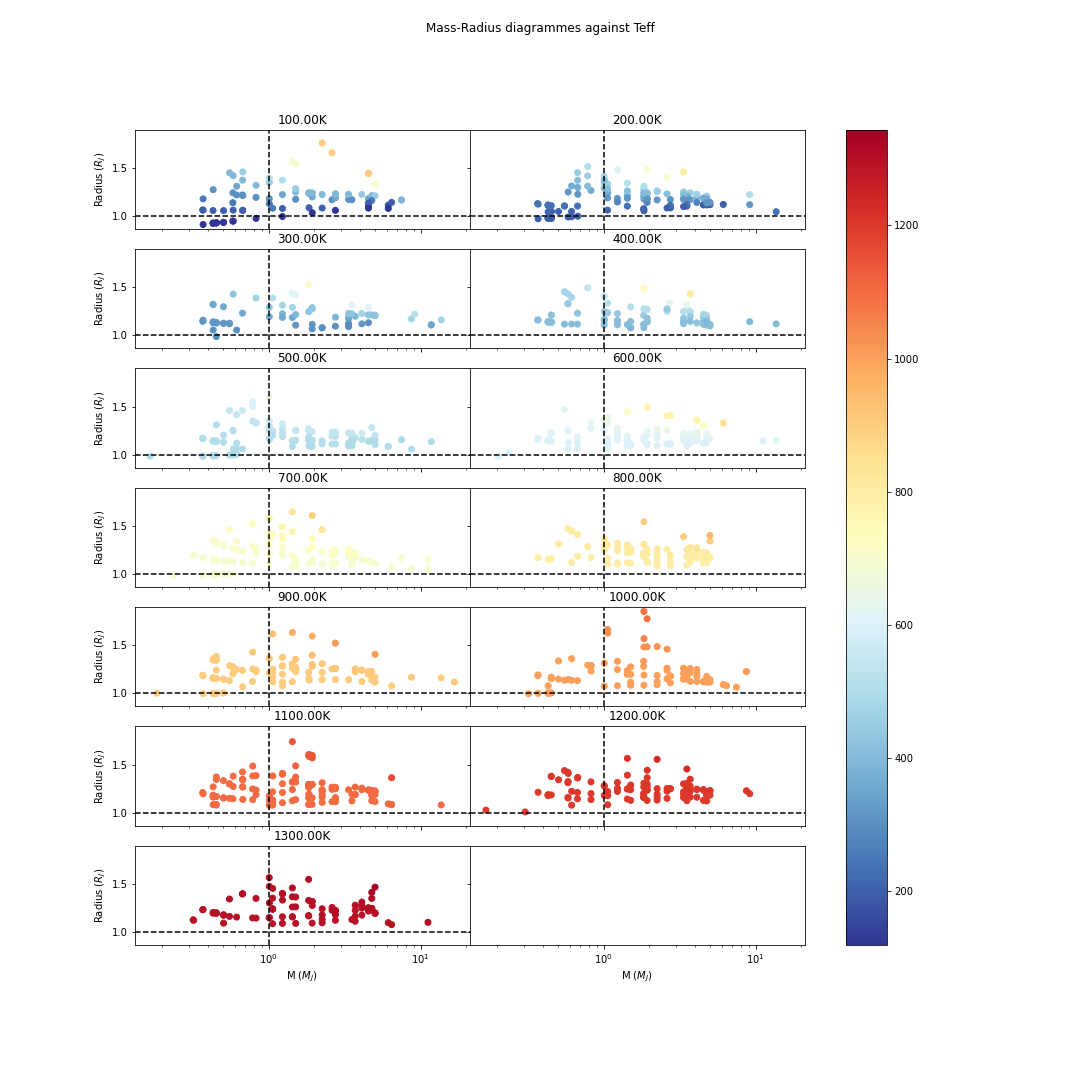
\includegraphics[width=0.48\textwidth]{Images/M_R_Teff.png}
    \caption{Mass Radius plots for different irradiation temperatures, plotted with effective temperature in color axis}
    \label{fig:M_R_Teff}
\end{figure}

\Cref{fig:T_int_R_Tirr} Links the results from \cref{fig:M_R_Tint} so that irradiation temperatures can be compared. We see that in general, higher irradiation temperatures lead to higher radii at a given internal temperature. There seems to be at higher mass a potential inversion of this as internal temperature increases, this however requires further precision to confirm. \par

\begin{figure}
    \centering
    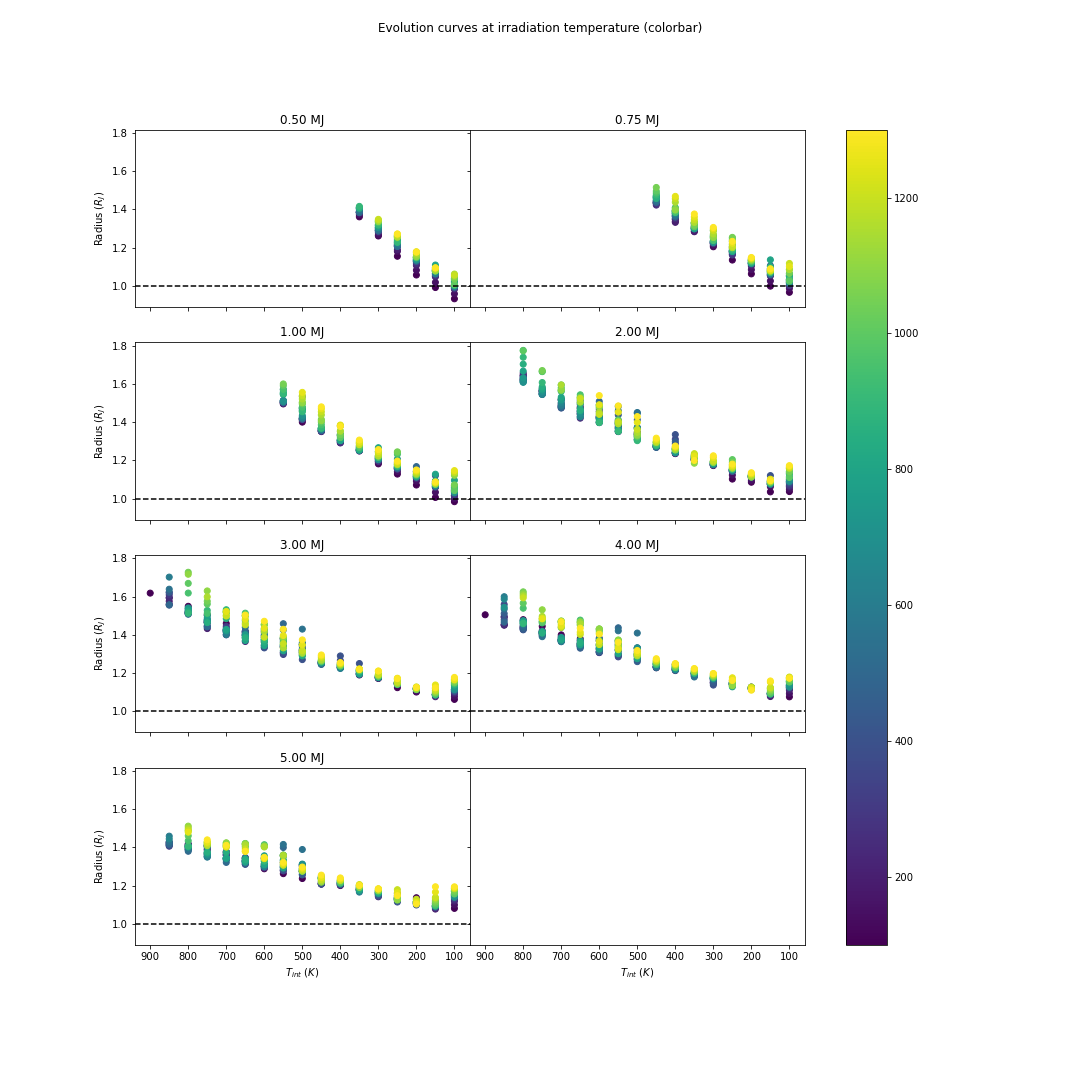
\includegraphics[width=0.48\textwidth]{Images/T_int_R_Tirr.png}
    \caption{Radius as a function of internal temperature for various planetary masses, plotted with irradiation temperatures in color axis}
    \label{fig:T_int_R_Tirr}
\end{figure}

\Cref{fig:T_eff_R_Tirr} is similar to \cref{fig:T_int_R_Tirr}, however we use the effective temperature instead of the internal temperature. This plot is a direct consequence of \cref{fig:M_R_Teff} where we see that for high irradiation temperatures, the effective temperature is equivalent to the irradiation temperature. \par

\begin{figure}
    \centering
    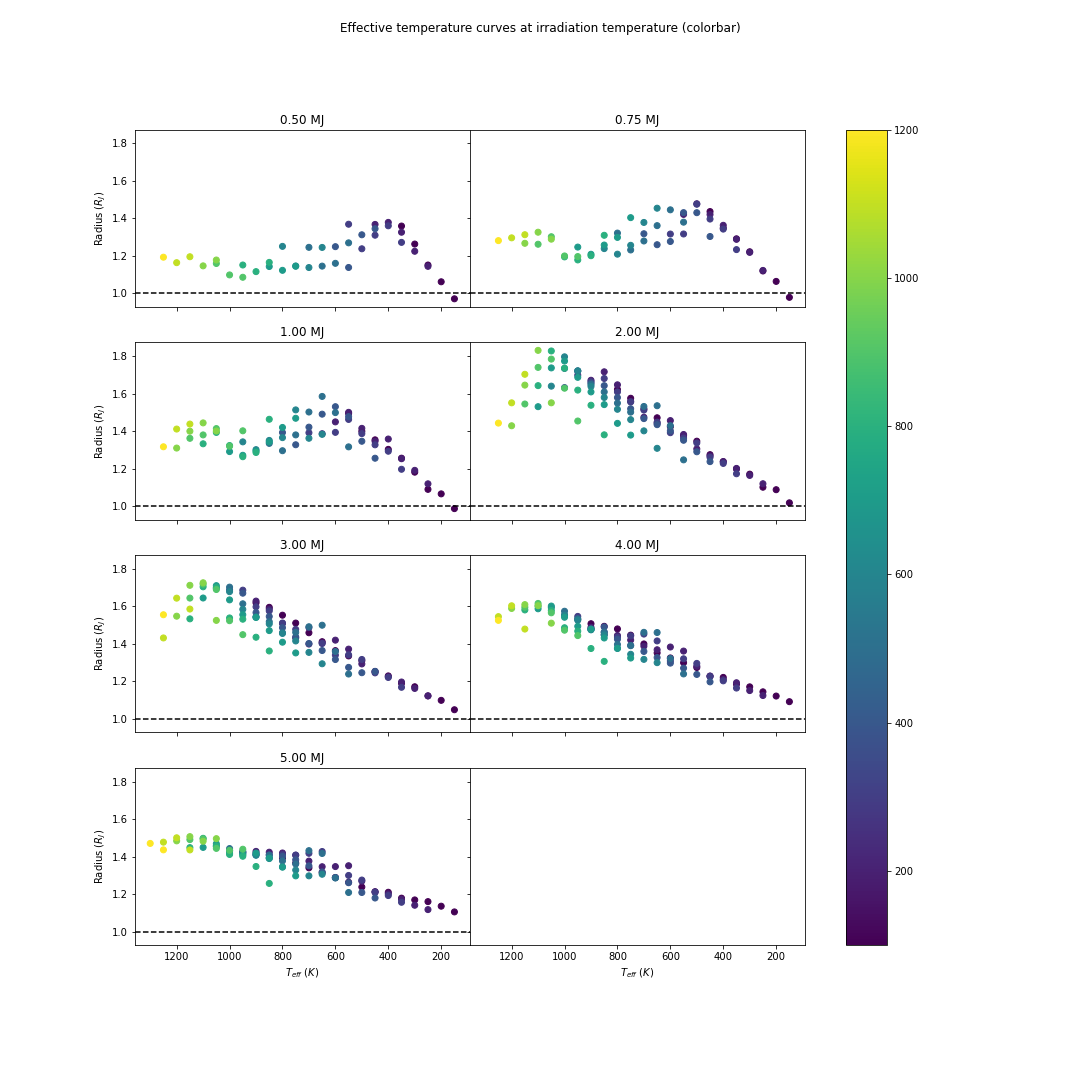
\includegraphics[width=0.48\textwidth]{Images/T_eff_R_Tirr.png}
    \caption{Radius as a function of effective temperature for various planetary masses, plotted with irradiation temperatures in color axis}
    \label{fig:T_eff_R_Tirr}
\end{figure}

\Cref{fig:SR} Shows how the spectral radiosity varies with internal temperature (color gradient) and irradiation temperature. We see that as temperature increases (internal and irradiation) individual spectral features at different wavelengths gradually fade away. \par

\begin{figure}
    \centering
    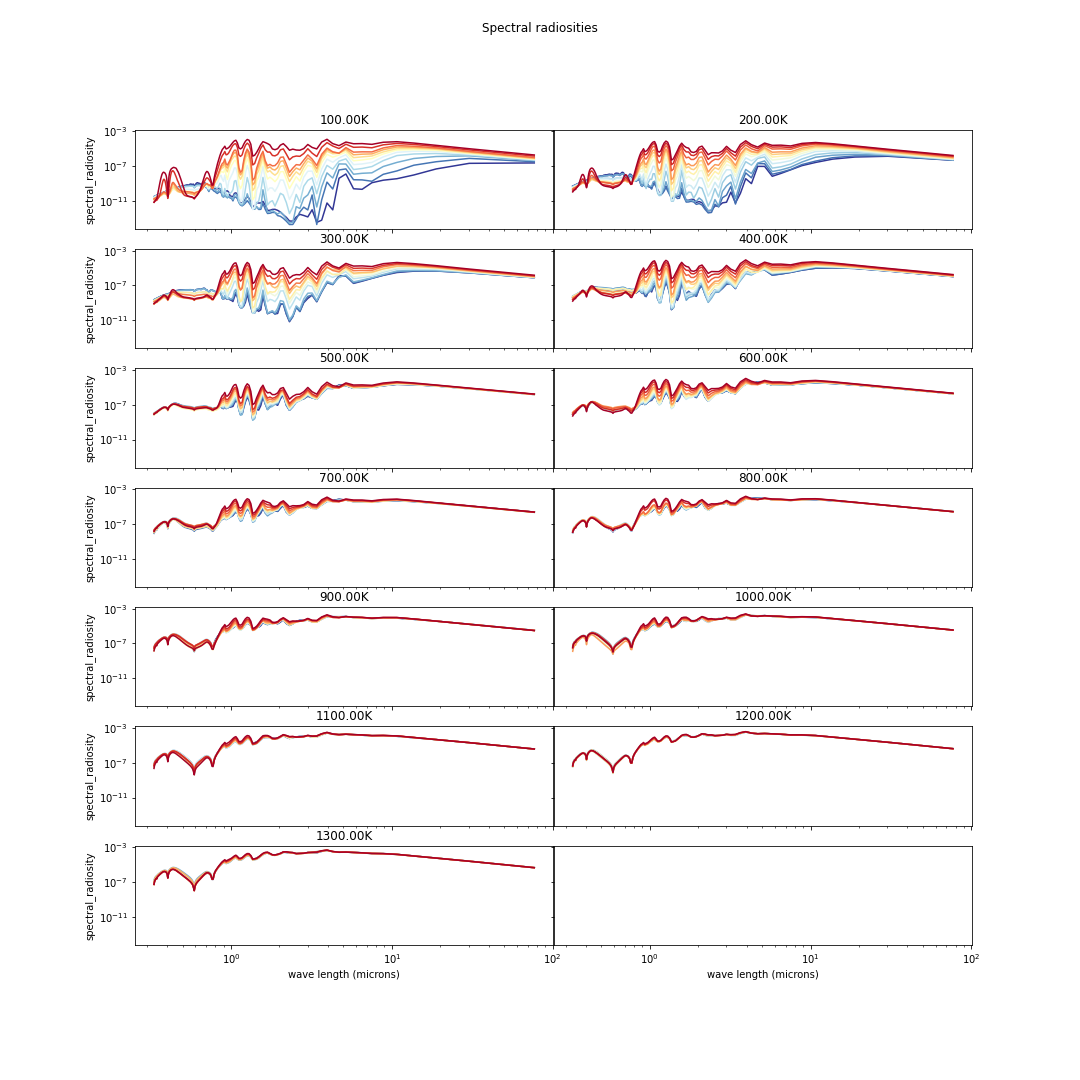
\includegraphics[width=0.48\textwidth]{Images/spectral_radiosity.png}
    \caption{Spectral radiosities for various Irradiation temperatures and internal temperatures (color gradient)}
    \label{fig:SR}
\end{figure}